\section{Esercizio 6}

Si consideri un reticolo di diffrazione con $N=5$ fenditure. Si supponga di avere uno schermo a distanza $L$ dalla sorgente. Si simuli con un programma lo spettro di intensità $\mathpzc{I}$ su questo schermo. Per un campione di $50000$ eventi si disegni un istogramma sperimentale di $\mathpzc{I}$ con \textsl{bin-width} $\Delta x$ scelta opportunamente. A questo punto si applichi uno \textsl{smearing} gaussiano con $\sigma =c\Delta x$ ($0<c<10$) e si discuta il relativo effetto in funzione della scelta di $c$. Applicando una delle tecniche di regolarizzazione viste a lezione si faccia l'\textsl{unfolding} delle distribuzioni sperimentali così costruite, discutendo la distribuzione ricostruita (si può ricorrere al package \texttt{RooUnfold} di \texttt{ROOT} o simili alternative).\\

\[* * * \] \medskip

\noindent Si è considerato l'esperimento schematizzato in \figurename~\ref{fig:SetupDiffraction}, notoriamente ben descritto dalla teoria diffrattiva di campo lontano ({diffrazione di Fraunhofer}). Tale modello prevede la seguente legge per l'intensità raccolta sullo schermo:

\begin{equation}
\mathpzc{I}(\vartheta) = \mathpzc{I}_0 \left(\frac{\sin(\beta\vartheta)}{\beta\vartheta}\right)^2\left(\frac{\sin (\!N\!\alpha \vartheta)}{\alpha\vartheta}\right)^2,
\label{eq:Fraunhofer}
\end{equation}

\noindent dove

\begin{itemize}
	\item[-] $\vartheta$ è l'angolo d'incidenza della luce sullo schermo ($\vartheta = 0$ definisce l'asse ottico);
	\item[-] $\alpha = \frac{ka}{2}$, con $a$ spaziatura fra le $N$ fenditure;
	\item[-] $\beta = \frac{kb}{2}$, con $b$ larghezza di ogni singola fenditura;
	\item[-] $k$ è il vettore d'onda della luce monocromatica immessa nel sistema ottico.\\
\end{itemize}

\vfill

\begin{figure}[h!]
	\centering
	\caption{Apparato per la rivelazione di profili diffrattivi di campo lontano. }
	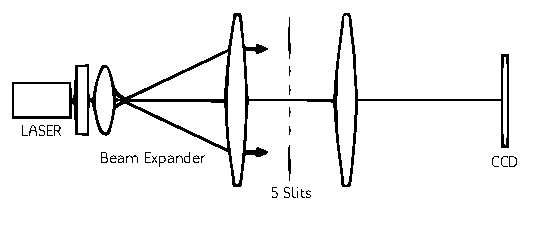
\includegraphics[width=.8\linewidth, trim={0 0 0 0.2cm}, clip]{Immagini/SetupFraunhofer}
	\label{fig:SetupDiffraction}
\end{figure}

\vfill

\noindent Ponendo in particolare $\mathpzc{I}_0=1$, $\alpha=1$, $\beta = 1/2$ e $N=5$ si ottiene il profilo spettrale tracciato in \figurename~\ref{fig:FraunhoferTheory}(a).\\

\noindent Per generare un campione distribuito secondo tale legge si è pensato di utilizzare la versione \emph{`hit or miss'} della tecnica Montecarlo: il metodo non è particolarmente efficiente ma di contro risulta estremamente flessibile nel caso di densità di probabilità inusuali.

\vfill

\newpage

\noindent L'algoritmo per la simulazione della generica densità $g(x)$ può essere sintetizzato nei seguenti passi:

\begin{enumerate}
	\item Generazione di un numero casuale $u$, estratto con probabilità uniforme nel dominio di $g$.
	\item Generazione di un numero casuale $y$, indipendente da $u$ ed estratto uniformemente dall'intervallo~$(0, \max[g(x)])$.
	\item Criterio \emph{`hit or miss'}: si "accetta" $u$ se $y < g(u)$; in caso contrario lo si scarta.
	\item Reiterazione \emph{ad libitum} del punto (1).
\end{enumerate}

\noindent La famiglia $\{u\}$ così ottenuta sarà distribuita secondo la densità $g$, dal momento che per ogni valore $u$ generato al passo (1) la probabilità di accettarlo è chiaramente proporzionale a $g(u)$. \\

\noindent In \figurename~\ref{fig:TheoryVsMontecarlo}(b) è riportato un istogramma degli eventi generati tramite algoritmo \emph{`hit or miss'}, con sovrapposta la curva teorica $\mathpzc{I}(\vartheta)$. Al netto di un piccolo \emph{bias} rigido (di origine ignota) sulla posizione dei picchi, i dati generati sembrano riprodurre con buona accuratezza lo spettro d'intensità desiderato. \\

\[* * * \] \medskip

\captionsetup*[subfigure]{position=top}
\begin{figure}
	\centering
	\caption{(a) Grafico dello spettro di intensità di Fraunhofer in funzione dell'angolo.\\
		(b) Confronto con l'istogramma degli eventi Montecarlo generati.}
	\subfloat[]{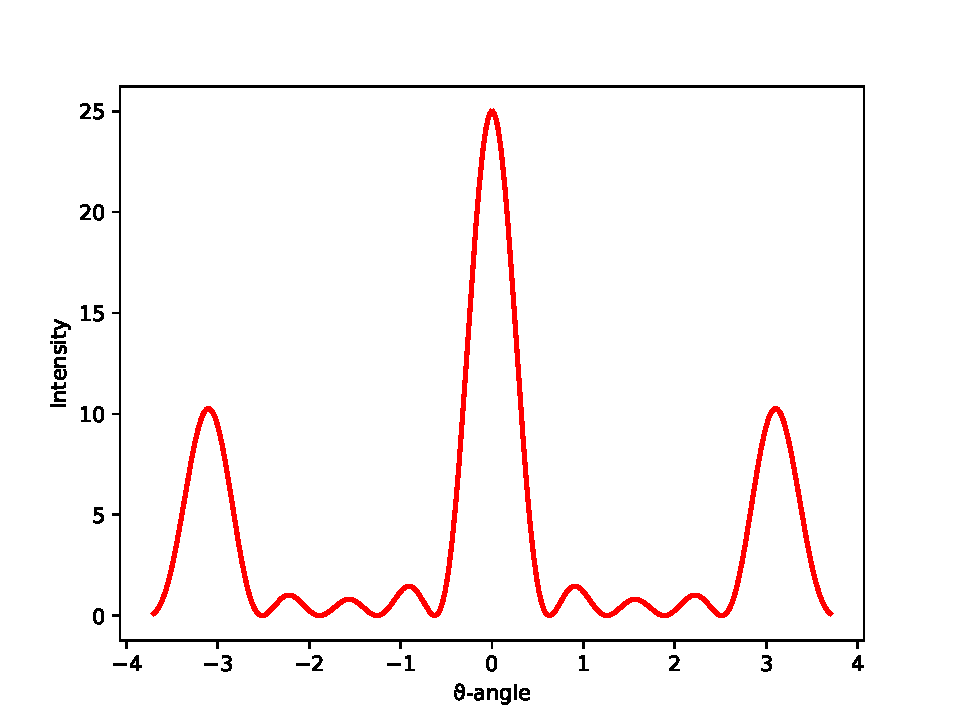
\includegraphics[width=0.8\linewidth,trim={0 0 0 1.4cm}, clip]{Immagini/Fraunhofer_Theory}}\label{fig:FraunhoferTheory}
	\subfloat[]{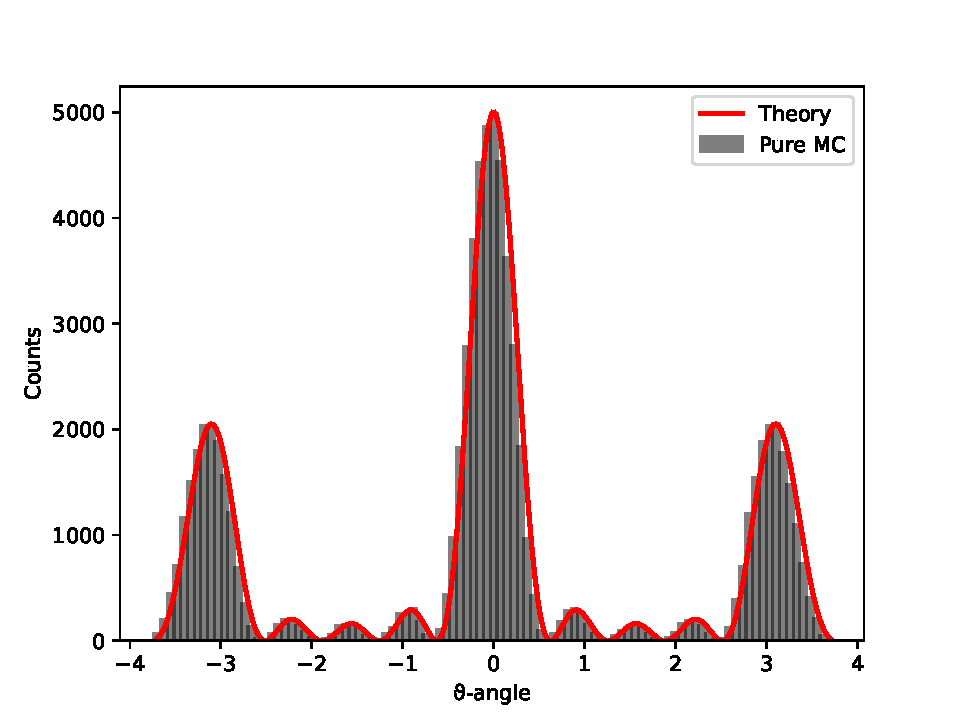
\includegraphics[width=0.8\linewidth,trim={0 0 0 1.4cm}, clip]{Immagini/TheoryVsMontecarlo}}\label{fig:TheoryVsMontecarlo}
\end{figure}

\noindent I dati rappresentati in \figurename~\ref{fig:TheoryVsMontecarlo}(b) simulano tuttavia solo la luce incidente sul rivelatore, non il segnale effettivamente misurato. In generale quest'ultimo viene in certa misura distorto dalla risposta spettrale del sistema di rivelazione. Chiamati $u(x)$ il segnale "vero" che incide sul rivelatore e $y(x)$ il segnale misurato, nell'assunzione che la risposta in frequenza dello strumento sia lineare possiamo dunque scrivere:

\begin{equation}
y(x_1) = \int_{-\infty}^{+\infty} K(x_1,x_2)u(x_2)\mathop{dx_2},
\label{eq:linearResponse}
\end{equation}

\noindent dove $K(x_1,x_2)$ (detto \emph{kernel}) descrive interamente le caratteristiche di risposta lineare dell'apparato rivelatore.\\

\noindent In generale dunque il kernel associato al rivelatore ne incorpora tutte le informazioni relative a efficienza e limiti di risoluzione\footnote{Eventuali fondi introdotti durante la rivelazione non vengono descritti dal modello, trattandosi di effetti di risposta non lineare.}. In particolare una risoluzione finita introduce una probabilità non nulla di registrare erroneamente un eventi relativi al  bin $j$-esimo su un bin $i$-esimo, coerentemente con  l'incertezza associata alla misura. Pertanto, assumendo \emph{accettanza} ideale (tutti gli eventi vengano rivelati in qualche bin) e discretizzando l'equazione (\ref{eq:linearResponse}), otteniamo una relazione matriciale tra frequenze attese sullo schermo $\{\mu\}$ e frequenze effettivamente rivelate $\{\nu\}$:
 
\begin{equation}
\nu_j = \sum_{i} \left[\mathcal{M}_{ij} \mu_i\right],\enspace\mathcal{M}_{ij} = \mathbb{P}\{\text{"Migrazione di un evento dal bin $i$-esimo al bin $j$-esimo"}\}.
\end{equation}

\noindent La matrice $\{\{\mathcal{M}\}\}$ sarà ovviamente tale da preservare la norma dei vettori su cui è applicata.\\

\noindent Per aggiungere anche gli effetti di risoluzione finita alla nostra simulazione occorre dunque costruire opportunamente una matrice statistica che tenga conto della migrazione aleatoria tra i bin. Per fare ciò introduciamo uno \emph{smearing} gaussiano dei valori binnati, con deviazione standard $\sigma = c\Delta x$, dove $\Delta x$ indica la larghezza del singolo bin e la costante $c$ controlla il limite risolutivo da simulare.\\

 \noindent Lo smearing viene in particolare eseguito generando una sequenza casuale con distribuzione normale, per mezzo del comando \texttt{random.normal} incluso nel pacchetto \texttt{numpy} di \texttt{Phyton}\footnote{La documentazione relativa può essere consultata al seguente link: \href{https://docs.scipy.org/doc/numpy-1.15.0/reference/generated/numpy.random.normal.html}{\texttt{https://docs.scipy.org/doc/[...]/numpy.random.normal.html}}.}. Delle rappresentazioni in \emph{colormap discreta} delle matrici di smearing generate per diversi valori di $c$ sono riportate in \figurename~\ref{fig:SmearingMatrix}: i grafici mostrano delle matrici pressocché simmetriche, come ci si aspetta smussando secondo una distribuzione pari rispetto al valor medio.
 
\captionsetup*[subfigure]{position=bottom}
\begin{figure} 
	\centering
	\caption{Rappresentazioni in \emph{colormap} delle matrici di smearing generate per diversi valori di $\sigma$.}
	\subfloat[$\enspace\sigma = 0.3\times\Delta x$]{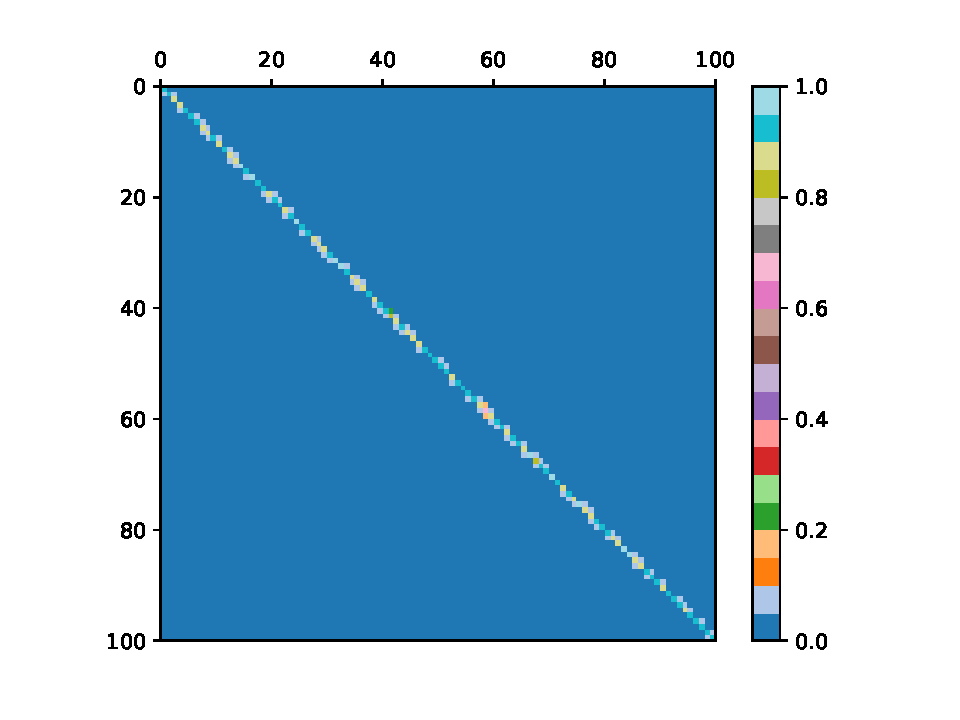
\includegraphics[width = .45\textwidth,trim={1cm 0 1cm 0}, clip]{Immagini/SmearingMatrix03.pdf}}
	\subfloat[$\enspace\sigma = 0.5\times\Delta x$]{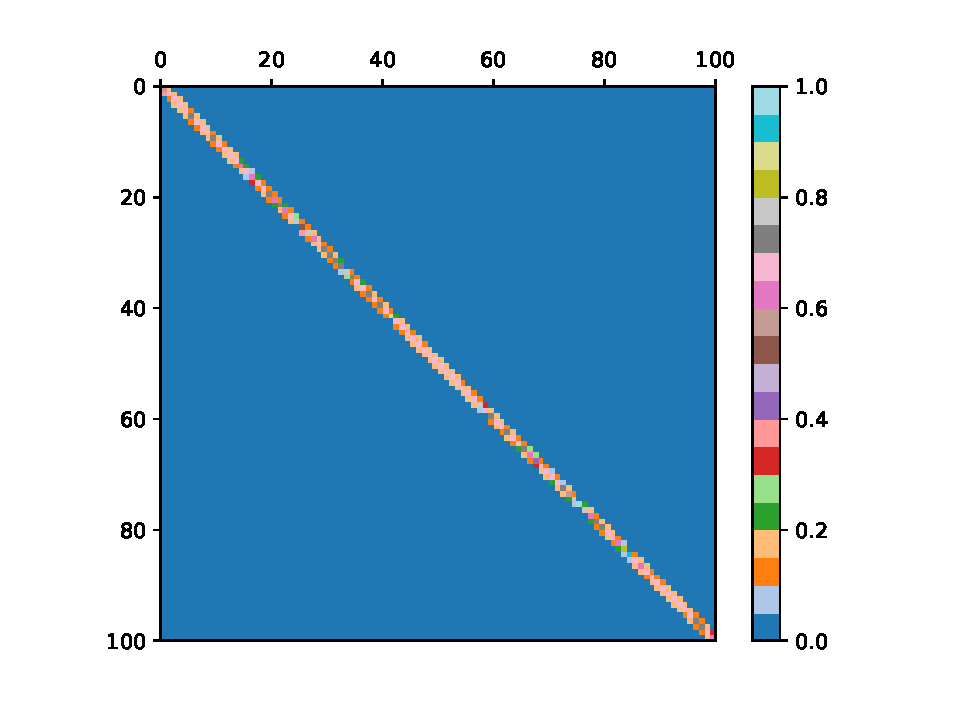
\includegraphics[width = .45\textwidth,trim={1cm 0 1cm 0}, clip]{Immagini/SmearingMatrix05.pdf}}\\
	\subfloat[$\enspace\sigma = 1.0\times\Delta x$]{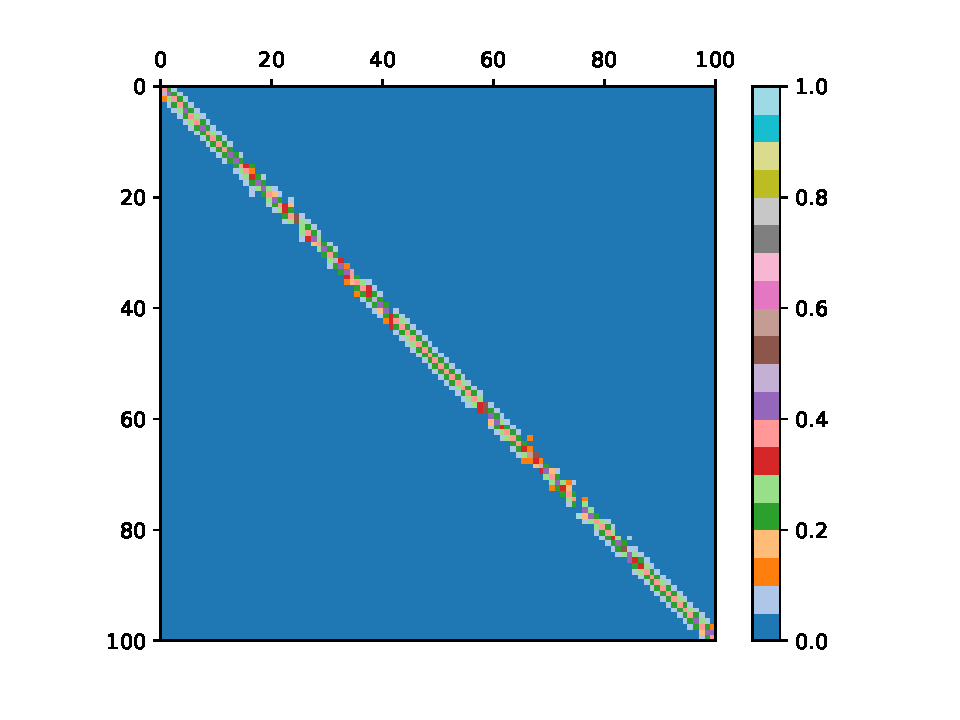
\includegraphics[width = .45\textwidth,trim={1cm 0 1cm 0}, clip]{Immagini/SmearingMatrix1.pdf}}
	\subfloat[$\enspace\sigma = 2.0\times\Delta x$]{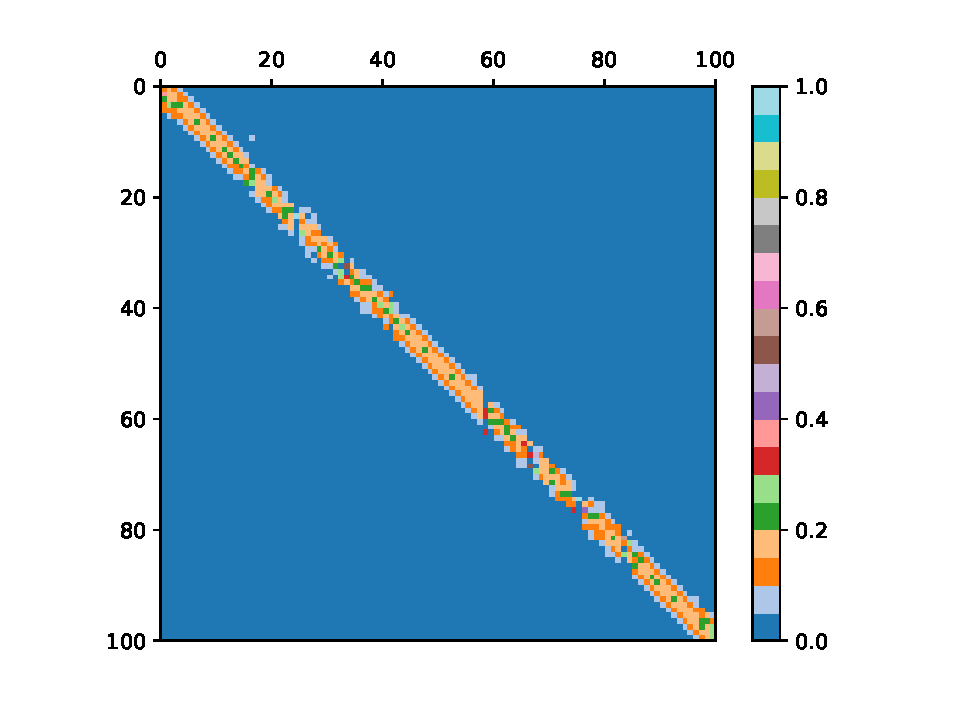
\includegraphics[width = .45\textwidth,trim={1cm 0 1cm 0}, clip]{Immagini/SmearingMatrix2.pdf}} \\
	\subfloat[$\enspace\sigma = 5.0\times\Delta x$]{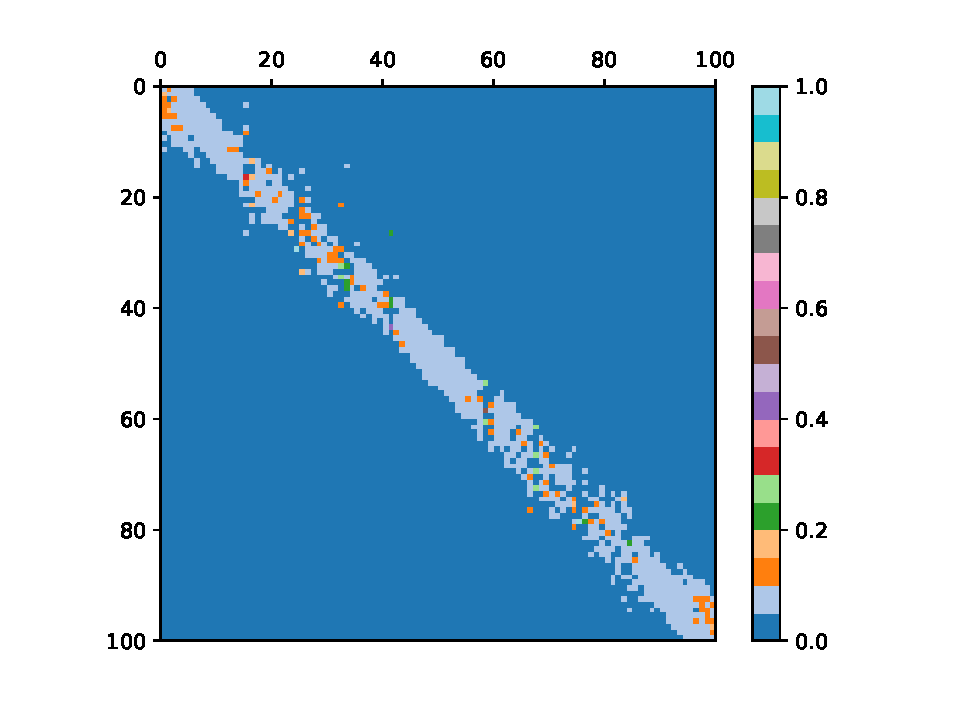
\includegraphics[width = .45\textwidth,trim={1cm 0 1cm 0}, clip]{Immagini/SmearingMatrix5.pdf}}
	\subfloat[$\enspace\sigma = 9.0\times\Delta x$]{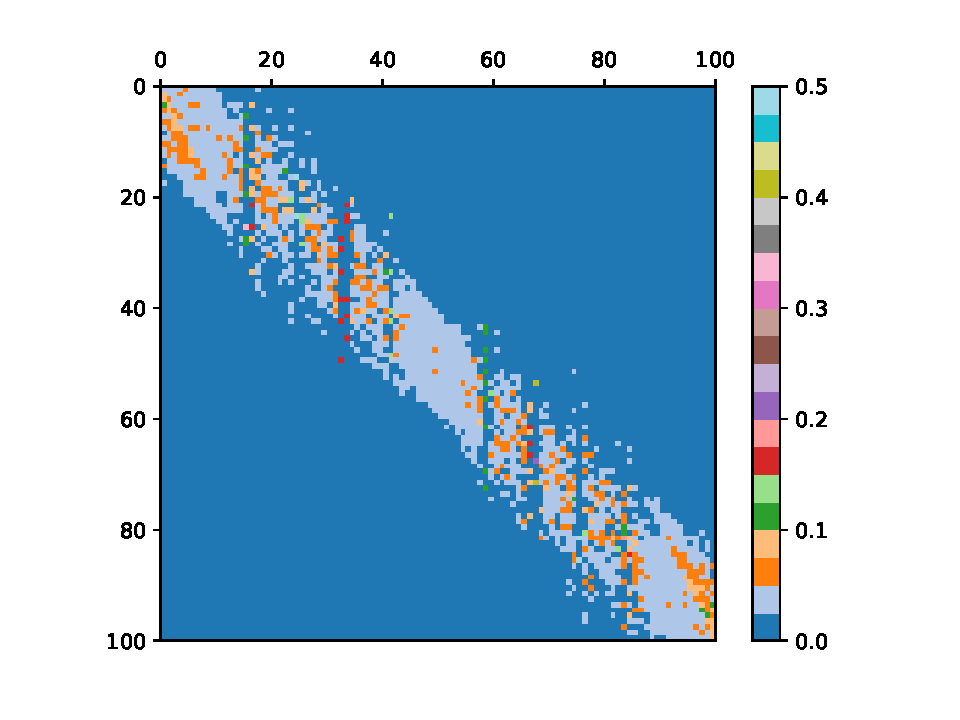
\includegraphics[width = .45\textwidth,trim={1cm 0 1cm 0}, clip]{Immagini/SmearingMatrix9.pdf}}
	\label{fig:SmearingMatrix}
\end{figure}

\newpage

\noindent In \figurename~\ref{fig:TrueVsSmeared} sono riportati gli istogrammi relativi ai diversi livelli di smearing operato sulla simulazione Montecarlo "pura". Osserviamo che al crescere del parametro di smearing $c$ si ha una maggiore migrazione tra i bin, con il progressivo svuotamento dei picchi fino alla totale sparizione di quelli minori, coperti dal fondo prodotto dalle code di quelli principali. Tali risultati ben corrispondono a ciò che ci si aspetta da una misura spettrale poco risoluta.\\

\[* * * \] \medskip

\noindent Resta infine da simulare l'operazione inversa, ossia l'\emph{unfolding} dei dati sperimentali misurati e quindi convoluti con il kernel di risposta del rivelatore. Lo scopo è di ottenere un segnale che riproduca il più possibile il profilo d'intensità incidente sullo schermo, ossia dei dati direttamente confrontabili con il modello teorico da testare. Assumeremo dunque i dati precedentemente sottoposti a smearing come input sperimentale da analizzare e confronteremo il risultato deconvoluto con l'intensità teorica predetta dal modello di Fraunhofer.\\

\noindent Il metodo di unfolding presentato è quello dei cosiddetti "coefficienti di correzione \emph{bin-by-bin}".  Si tratta sostanzialmente di definire dei coefficienti correttivi per il valore di ciascun bin, basandosi su delle simulazioni di segnale puro e smussato analoghe a quelle presentate poco sopra. Formalmente, chiamate $T_i$ la frequenza attesa nel bin $i$-esimo per il segnale a monte della risposta strumentale, e $R_i$ la frequenza attesa per i conteggi effettivamente raccolti nel \emph{pixel} $i$-esimo del rivelatore (entrambe quantità simulabili per mezzo di generatori pseudo-casuali), definiamo i coefficienti di correzione \emph{locali}\footnote{La matrice inversa $\{\{\mathcal{M}^{-1}\}\}$, che se nota ci darebbe l'unfolding esatto dei dati, rappresenta una relazione \emph{non locale} fra i bin, in quanto il valore da assegnare al bin $i$-esimo dipende in linea di principio dal valore di anche tutti gli altri. Il metodo dei coefficienti di correzione invece definisce per ogni bin un fattore correttivo che dipende solo dal valore misurato sul medesimo bin. Va da sé che tale metodo può essere ritenuto affidabile solo per tassi di migrazione inter-bin estremamente ridotti.}

\begin{equation}
C_i = \frac{T_i}{R_i},
\end{equation}

\noindent per mezzo dei quali si potrà stimare la distribuzione $U_i$, deconvoluta a partire dai dati sperimentali $D_i$, applicando la semplice relazione di proporzione

\begin{equation}
U_i = C_i D_i.
\end{equation}

\noindent Inoltre, se il numero di eventi raccolti su ciascun bin è sufficientemente elevato, a tale stima può essere associata una deviazione standard data da

\begin{equation}
\sigma(U_i) = C_i \sqrt{D_i}.
\end{equation}

\noindent Il predittore $U_i$ ha dunque il pregio di avere una varianza piuttosto ridotta, ma al prezzo di introdurre - perlomeno nel caso generale - un bias sul valor medio dei dati ricostruiti. In particolare è facile dimostrare che

\begin{equation}
\mathpzc{B}(U_i) = \left(\frac{T_i}{R_i}\Biggl|^{\mathrm{MC}} \!\!\!\!- \enspace\frac{\mu_i}{D_i}\right) = C_i^{^\mathrm{MC}} \!\! - \enspace\frac{\mu_i}{D_i},
\end{equation}

\noindent ossia l'unfolding non introduce bias a patto che la simulazione Montecarlo riproduca in maniera fedele la fisica dell'esperimento e della rivelazione. \\

\noindent I risultati dell'unfolding sono riportati in \figurename~\ref{fig:Unfolded}, comparati con il profilo spettrale dato dalla (\ref{eq:Fraunhofer}). Osserviamo che, anche per i valori più grandi di $c$, la ricostruzione appare qualitativamente corretta, con ottima sovrapposizione\footnote{Resta naturalmente il piccolo bias rigido che avevamo notato già sulla simulazione Montecarlo "pura".} tra istogramma dei dati deconvoluti e curva teorica.

\begin{figure} 
	\centering
	\caption{Confronto tra segnale "vero" e simulazioni di segnale misurato, ottenute per smussamento gaussiano, con~deviazione standard via via crescente.}
	\subfloat[$\enspace\sigma = 0.3\times\Delta x$]{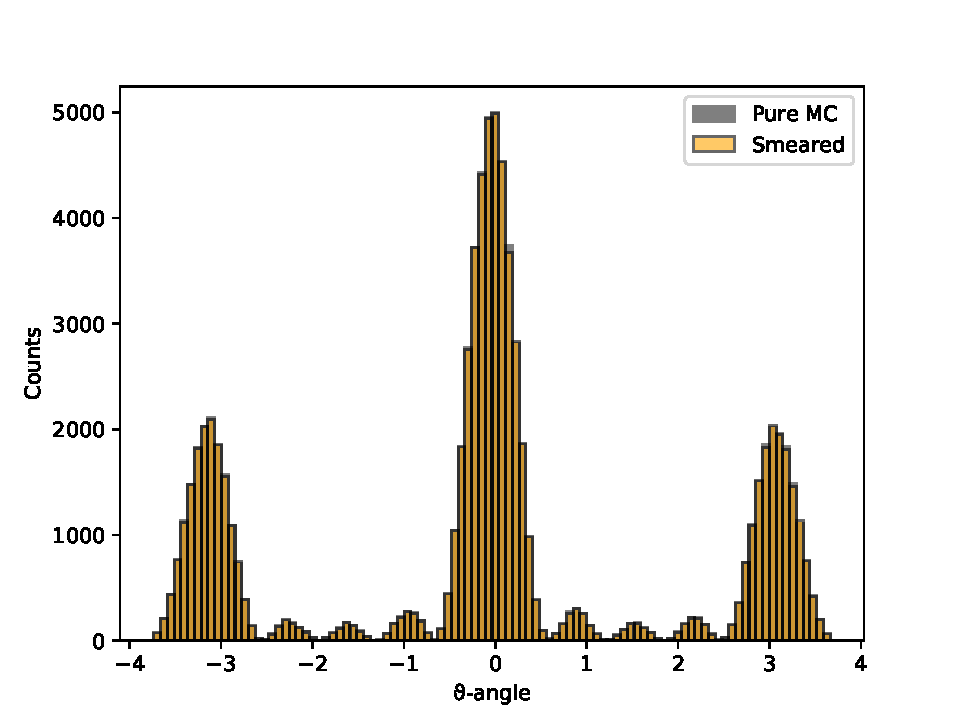
\includegraphics[width = .5\textwidth,trim={0 0 0 1.2cm}, clip]{Immagini/TrueVsSmeared03.pdf}}
	\subfloat[$\enspace\sigma = 0.5\times\Delta x$]{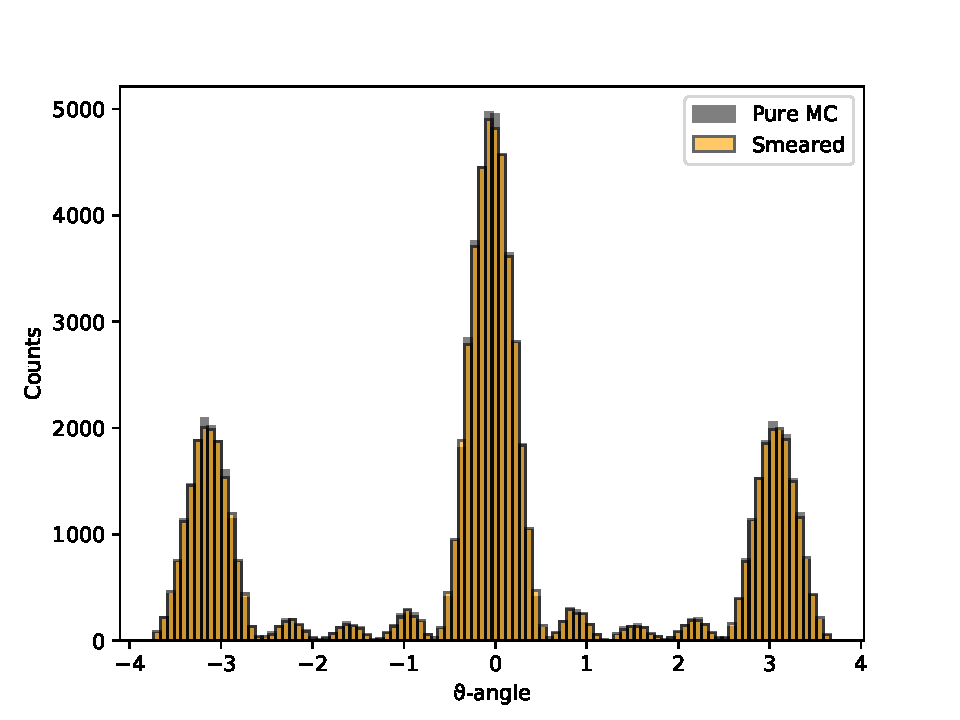
\includegraphics[width = .5\textwidth,trim={0 0 0 1.2cm}, clip]{Immagini/TrueVsSmeared05.pdf}}\\
	\subfloat[$\enspace\sigma = 1.0\times\Delta x$]{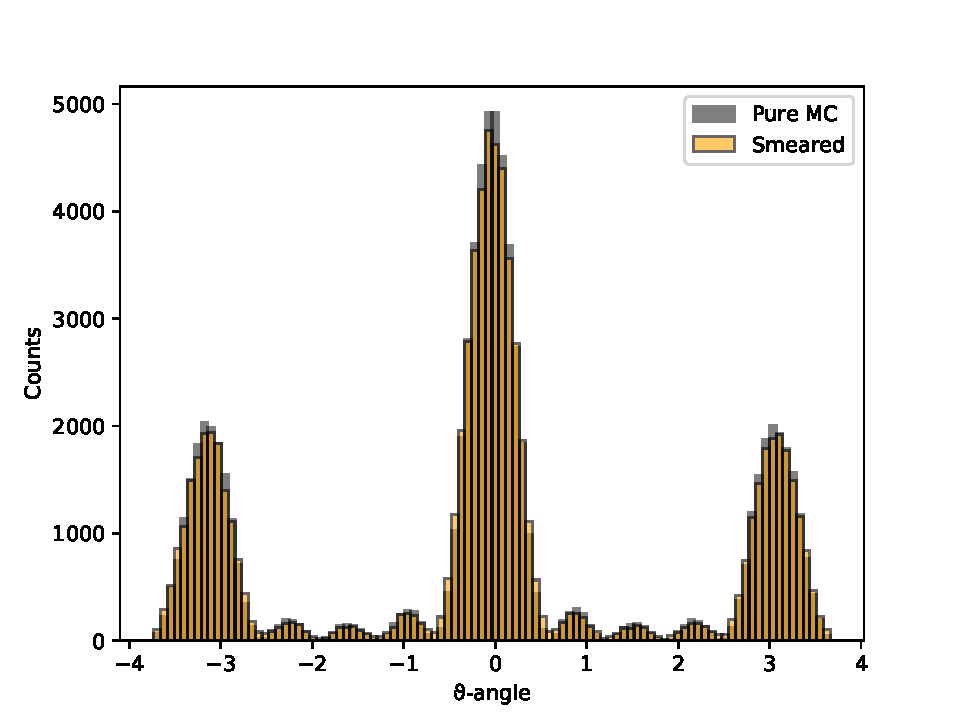
\includegraphics[width = .5\textwidth,trim={0 0 0 1.2cm}, clip]{Immagini/TrueVsSmeared1.pdf}}
	\subfloat[$\enspace\sigma = 2.0\times\Delta x$]{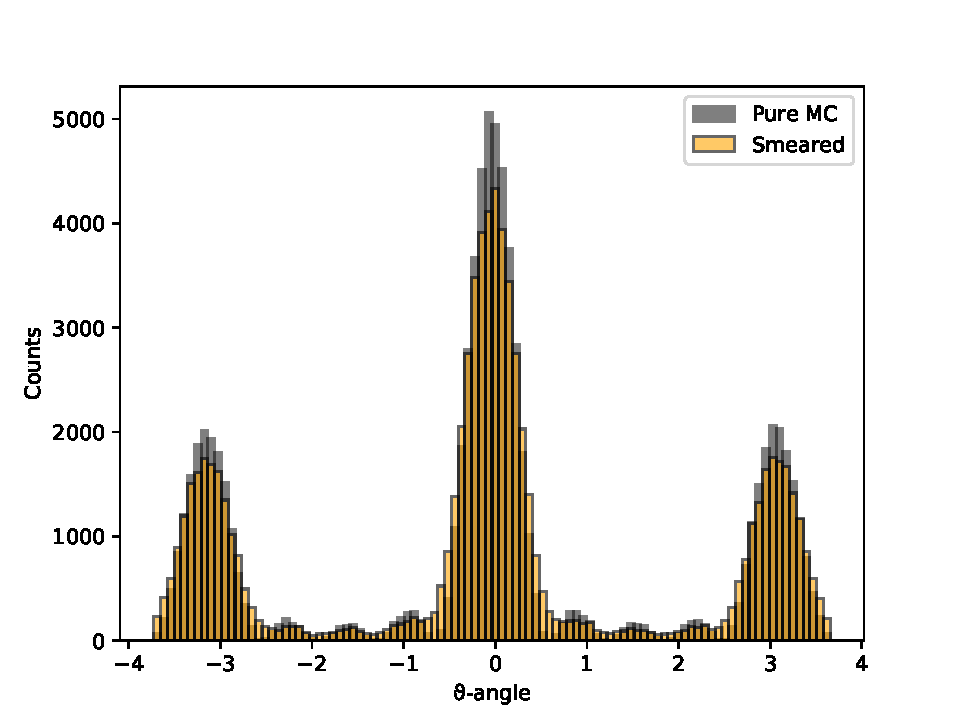
\includegraphics[width = .5\textwidth,trim={0 0 0 1.2cm}, clip]{Immagini/TrueVsSmeared2.pdf}} \\
	\subfloat[$\enspace\sigma = 5.0\times\Delta x$]{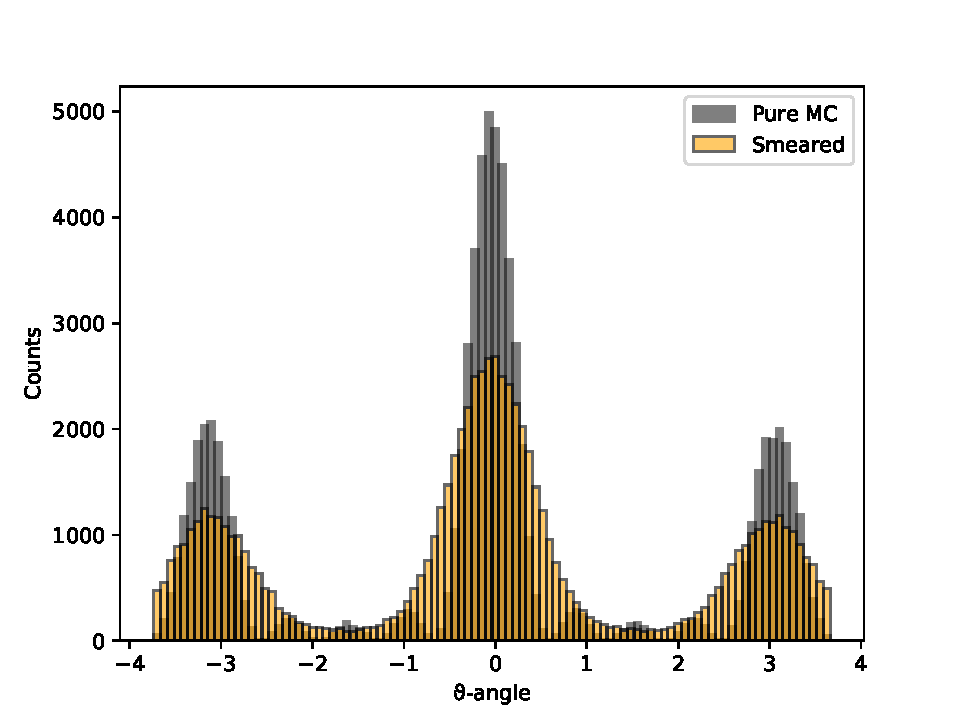
\includegraphics[width = .5\textwidth,trim={0 0 0 1.2cm}, clip]{Immagini/TrueVsSmeared5.pdf}}
	\subfloat[$\enspace\sigma = 9.0\times\Delta x$]{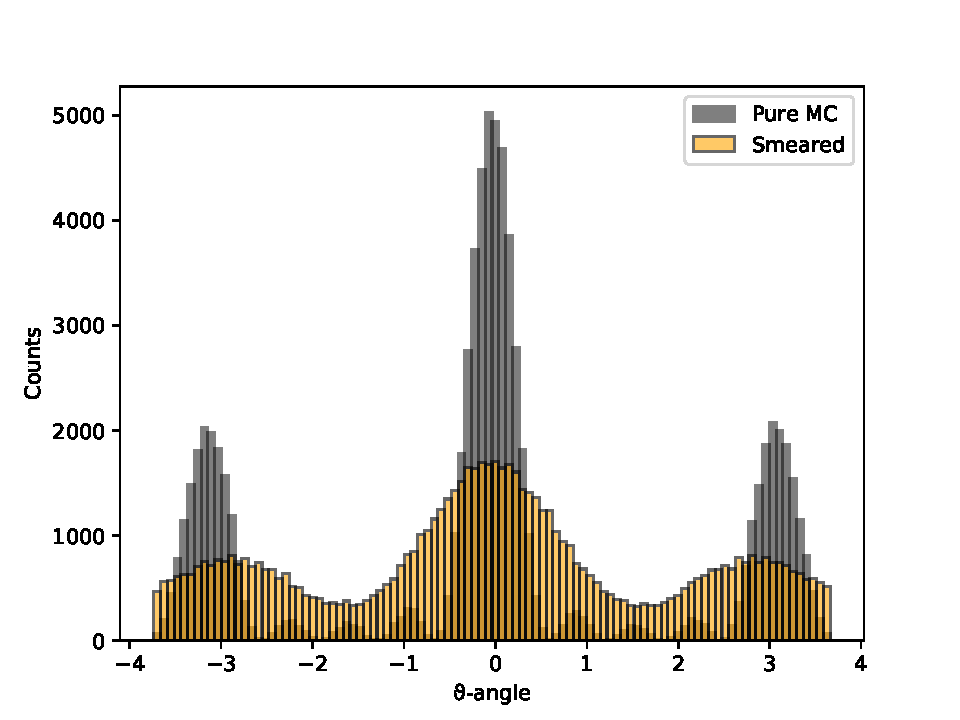
\includegraphics[width = .5\textwidth,trim={0 0 0 1.2cm}, clip]{Immagini/TrueVsSmeared9.pdf}}
	\label{fig:TrueVsSmeared}
\end{figure}

\begin{figure} 
	\centering
	\caption{Unfolding delle distribuzioni sperimentali simulate tramite smearing gaussiano di varianza $\sigma^2$ e~confronto con il profilo d'intensità teorico.}
	\subfloat[$\enspace\sigma = 0.3\times\Delta x$]{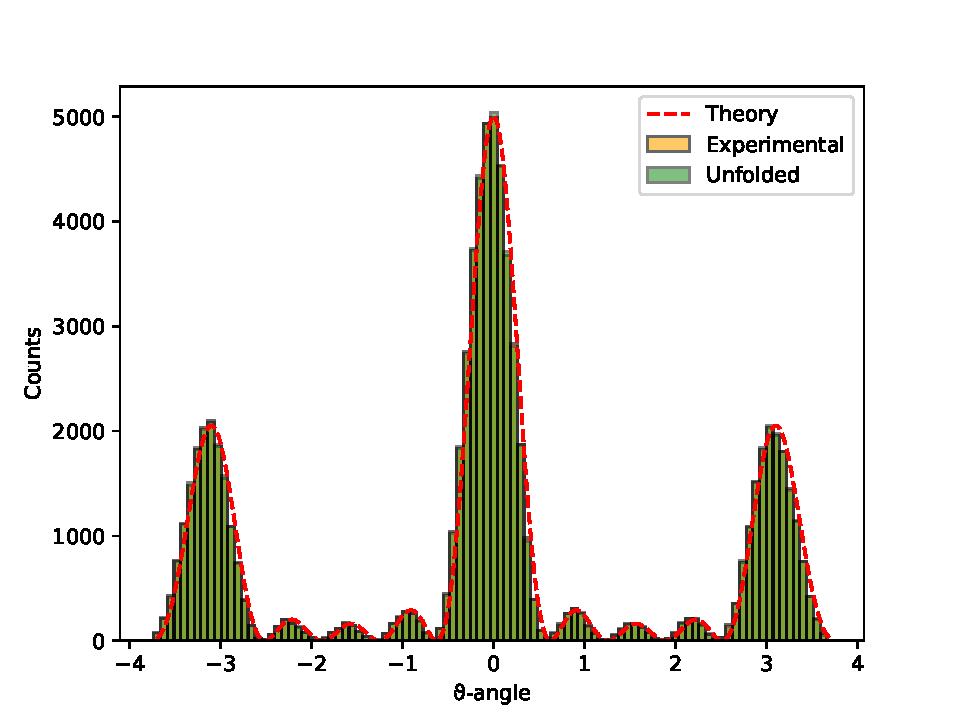
\includegraphics[width = .5\textwidth,trim={0 0 0 1.2cm}, clip]{Immagini/Unfolded03.pdf}}
	\subfloat[$\enspace\sigma = 0.5\times\Delta x$]{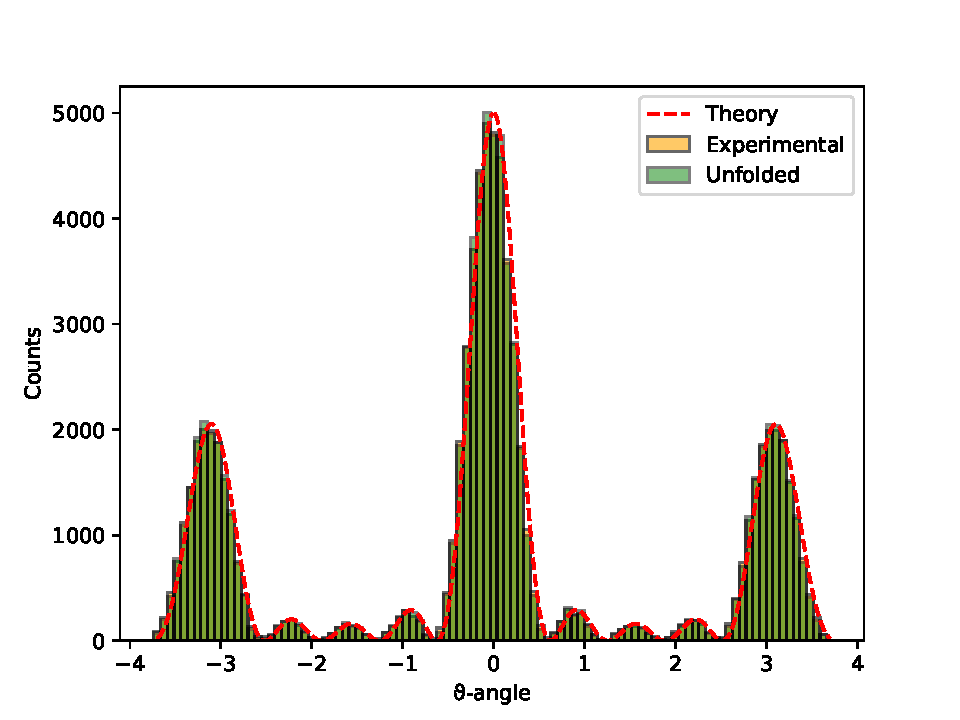
\includegraphics[width = .5\textwidth,trim={0 0 0 1.2cm}, clip]{Immagini/Unfolded05.pdf}}\\
	\subfloat[$\enspace\sigma = 1.0\times\Delta x$]{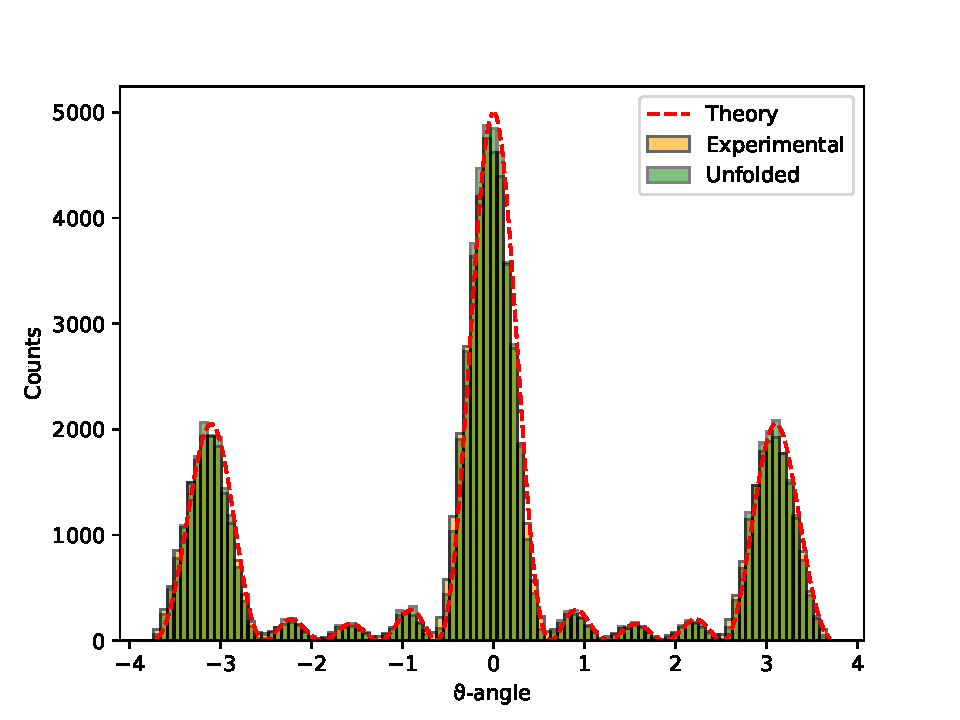
\includegraphics[width = .5\textwidth,trim={0 0 0 1.2cm}, clip]{Immagini/Unfolded1.pdf}}
	\subfloat[$\enspace\sigma = 2.0\times\Delta x$]{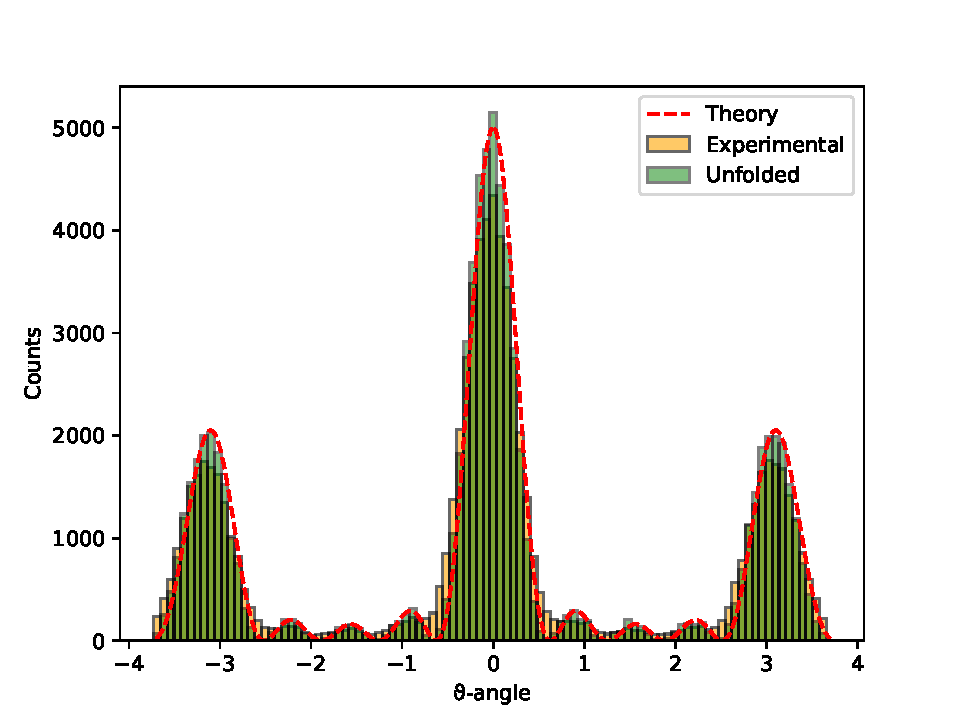
\includegraphics[width = .5\textwidth,trim={0 0 0 1.2cm}, clip]{Immagini/Unfolded2.pdf}} \\
	\subfloat[$\enspace\sigma = 5.0\times\Delta x$]{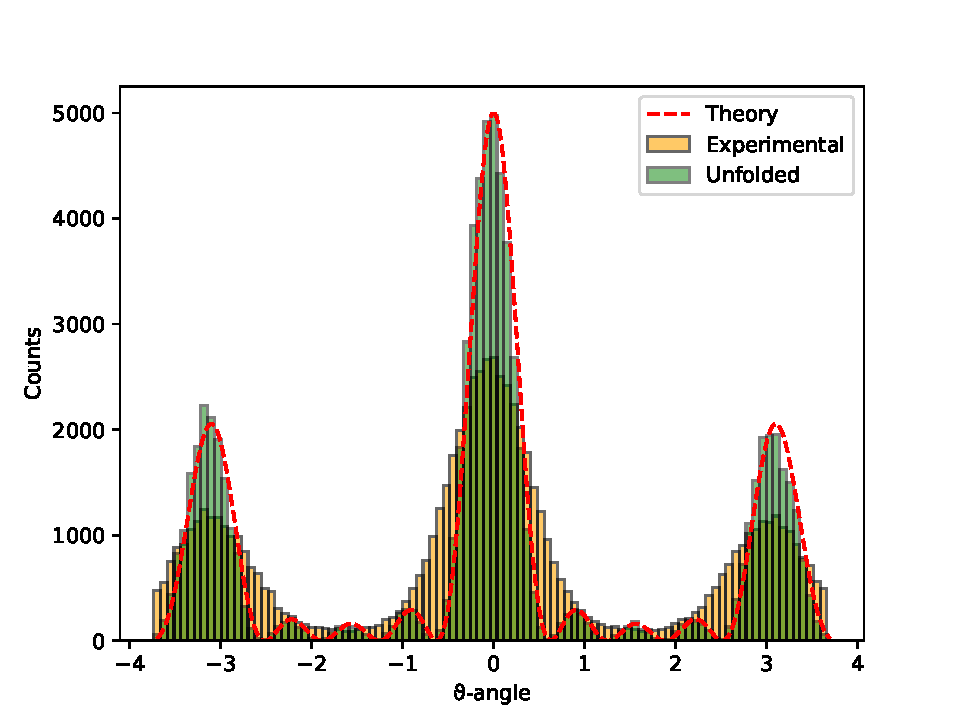
\includegraphics[width = .5\textwidth,trim={0 0 0 1.2cm}, clip]{Immagini/Unfolded5.pdf}}
	\subfloat[$\enspace\sigma = 9.0\times\Delta x$]{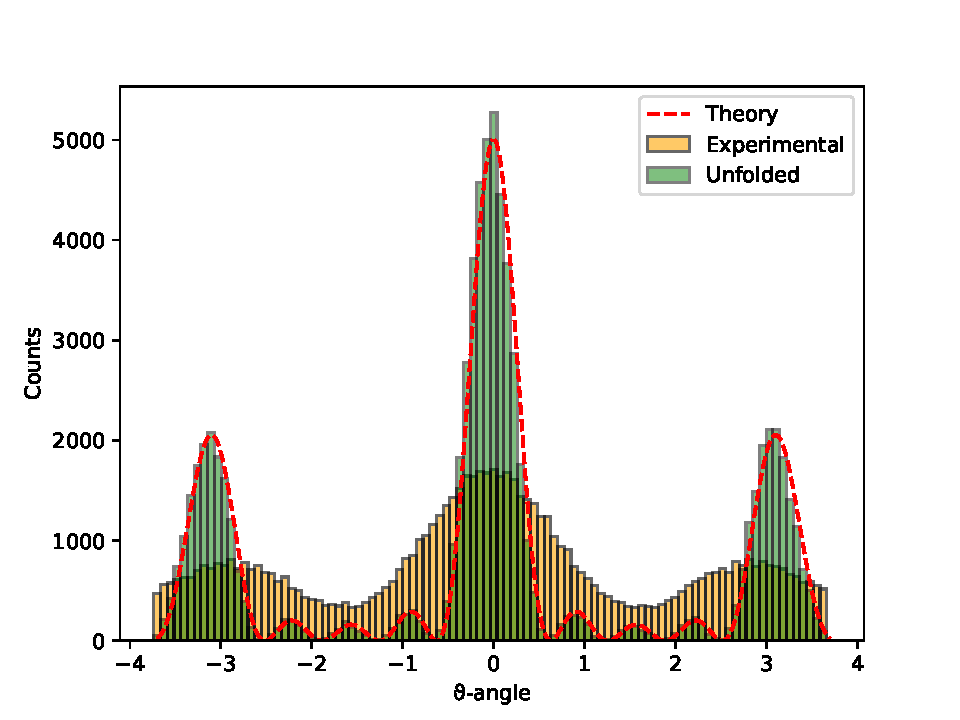
\includegraphics[width = .5\textwidth,trim={0 0 0 1.2cm}, clip]{Immagini/Unfolded9.pdf}}
	\label{fig:Unfolded}
\end{figure}

\newpage

\noindent Sono stati inoltre eseguiti dei test d'ipotesi alla Pearson (Cfr. pag.\pageref{PearsonTest}) per valutare quantitativamente la compatibilità statistica tra i dati ricostruiti per unfolding e la relativa distribuzione Montecarlo "pura" (che nella nostra simulazione rappresenta il segnale sperimentale non convoluto con la risposta del rivelatore). I risultati dei test, riportati di seguito in tabella, hanno evidenziato come in realtà la qualità dell'unfolding decresca fortemente con l'aumentare del parametro di smearing $c$, come del resto inevitabilmente ci si aspetta.

 \bgroup
\def\arraystretch{2}
\begin{center}
	\begin{tabular}{c||c|c}
		{Smearing Parameter} & Calculated $\chi^2$ & Pearson's Test \emph{p-value}\\  \hline
		$\enspace\sigma = 0.3\times\Delta x$ & $5.836227590882934$ & $9.9999999999999999\,\times\,10^{-1} $\\
		$\enspace\sigma = 0.5\times\Delta x$ & $46.07973100467730$ & $9.9999884304470930\,\times\,10^{-1} $\\
		$\enspace\sigma = 1.0\times\Delta x$ & $125.5552504111569$ & $3.6953389551196786\,\times\,10^{-2} $\\
		$\enspace\sigma = 2.0\times\Delta x$ & $163.9468296504027$ & $4.4389667615274120\,\times\,10^{-5} $\\
		$\enspace\sigma = 5.0\times\Delta x$ & $223.2895908776605$ & $1.374244096699173\,\times\,10^{-11} $\\
		$\enspace\sigma = 9.0\times\Delta x$ & $225.4725538157693$ & $7.343546495541846\,\times\,10^{-12}$\\

	\end{tabular}
\end{center}
\egroup

\medskip

\noindent Per concludere riportiamo per intero il codice utilizzato per la generazione, lo smearing e l'unfolding dei dati discussi:

\begin{lstlisting}[language=python, style=Pystyle, caption=\texttt{Python} code for Exercise 6 (Smearing and Unfolding routines), label=list:Diffraction, 	captionpos=b]
""" Standard Libraries """
import numpy as np
from pylab import *
from math import *

""" Pearson's Test Library """
from scipy.stats import chisquare 

## Fraunhofer Theory for Diffraction [N: #{apertures}]
def f(x):

	N = 5
	I0 = 1
	a = 1
	b = 0.5
	return I0*(np.sin(b*x)/(b*x))**2*np.sin(N*a*x)**2/np.sin(a*x)**2

## Smearing Parameter Choice [0 < c < 10]
c = 1

## First MC-simulation ['hit or miss'] to compute N_true
x1 = np.linspace(-3.7,-0.01,200)  # Have to decompose the domain to
x2 = np.linspace(0.01,3.7,200)    # eliminate the x = 0 singularity!
v = max(f(x1))

N_true = np.array([0])
while(sum(N_true==0)>=1): # Have to assure no bin results empty

	u = np.random.uniform(-3.7,3.7,500000)
	t = f(u)
	y = np.random.uniform(0,v,500000)
	boolean = y<t
	u = u[boolean]
	N_true,bin_edges1 = np.histogram(u,bins=100) # Pure Theoretical MC-Simulation

## Plotting 'Theory' and 'Theory Vs MC-Simulation'
half_bin = 0.5*(bin_edges1[len(bin_edges1)-1]-bin_edges1[len(bin_edges1)-2])
bin_values = bin_edges1[:-1]+half_bin
half_bin = 0.5*(bin_values[len(bin_values)-1]-bin_values[len(bin_values)-2])
bin_edges1 = np.append(bin_values-half_bin,bin_values[len(bin_values)-1]+half_bin)

plt.figure('Fraunhofer Theory')
plt.plot(x1,f(x1), color='r', linewidth=2)
plt.plot(x2,f(x2), color='r', linewidth=2)
plt.xlabel("$\vartheta$"'-angle')
plt.ylabel('Intensity')

plt.figure('TheoryVsMontecarlo')
plt.plot(x1,f(x1)*(2*3.7/half_bin), color='r', linewidth=2,label='Theory')
plt.plot(x2,f(x2)*(2*3.7/half_bin), color='r', linewidth=2)
plt.bar(bin_edges1[:-1],N_true,width=half_bin*2,color='k',alpha=0.5,edgecolor='k',label='Pure MC')
plt.xlabel("$\vartheta$"'-angle')
plt.ylabel('Counts')
plt.legend()

## Computing Smearing Matrix from Normal-Random-Generator [...from numpy library]
n = len(bin_values)
delta_x = half_bin*2
sigma = c*delta_x

M = np.zeros((n,n))
for j in range(0,n):
	if N_true[j] == 0:
		print('error')
	p = np.random.normal(bin_values[j],sigma,N_true[j])
	for k in range(0,len(p)):
		if p[k] < -3.7:                      #
			p[k] = p[k]+2*(bin_values[j]-p[k])  # Folding the tails in...
		if p[k] > 3.7:                       # ------------------------
			p[k] = p[k]-2*(p[k]-bin_values[j])  # 
	for i in range(0,n):
		M[i,j] = sum((p>bin_values[i]-half_bin) & (p<bin_values[i]+half_bin))/(N_true[j]*1.0)

N_smeared = np.matmul(M,N_true) # ROWxCOL product by numpy package

T = N_true      # For subsequent use
R = N_smeared   # ------------------

## Plotting Smearing Matrix [colormap]
fig, ax = subplots()
im = imshow(M, cmap=cm.tab20, vmin=M.min(), vmax=M.max(), extent=[0, 100, 100, 0])
cb = fig.colorbar(im)
ax.xaxis.tick_top()

## Second MC-simulation ['hit or miss'] to compute a new, independent, N_smeared [D != R]
N_true = np.array([0])
while(sum(N_true==0)>=1): # Have to assure no bin result empty

	u = np.random.uniform(-3.7,3.7,500000)
	t = f(u)
	y = np.random.uniform(0,v,500000)
	boolean = y<t
	u = u[boolean]
	N_true,bin_edges1 = np.histogram(u,bins=100) # Pure MC

n = len(bin_values)
delta_x = half_bin*2
sigma = c*delta_x

N_smeared = np.matmul(M,N_true) # Represents a 'Simulated Experiment' to unfold...

## Plotting 'True Signal Vs Detected Signal'
plt.figure('TrueVsSmeared')
plt.bar(bin_edges1[:-1],N_true,width=half_bin*2,color='k',alpha=0.5,edgecolor='k',label='Pure MC')
plt.bar(bin_edges1[:-1],N_smeared,width=half_bin*2,color='orange',alpha=0.6,edgecolor='k',label='Smeared')
plt.xlabel("$\vartheta$"'-angle')
plt.ylabel('Counts')
plt.legend()

D = N_smeared # For subsequent use

## 'Bin-By-Bin Correction Factors' and Unfolding
C = T/R
U = C*D
sigma_U = C*D**0.5
dev = abs(U-T)

for i in range(U.shape[0]):					#
	if dev[i] > 2.3548200*sigma_U[i]:	# Checking error bars...
	print('Unfolding FAILED!')				#

N_unfold = U

## Chi-square test [Pearson] with respect to the last pure simulation
chi,p = chisquare(N_unfold,N_true)
print('chi: ', chi)
print('p-value: ', p)

## Plotting 'Theory Vs Experimental Vs Unfolded Signal'
plt.figure('Unfolded')
plt.plot(x1,f(x1)*(2*3.7/half_bin), color='r', linewidth=1.5,linestyle='--',label='Theory')
plt.plot(x2,f(x2)*(2*3.7/half_bin), color='r', linewidth=1.5, linestyle='--')
plt.bar(bin_edges1[:-1],N_smeared,width=half_bin*2,color='orange',alpha=0.6,edgecolor='k',label='Experimental')
plt.bar(bin_edges1[:-1],N_unfold,width=half_bin*2,color='g',alpha=0.5,edgecolor='k',label='Unfolded')
plt.xlabel("$\vartheta$"'-angle')
plt.ylabel('Counts')
plt.legend()

## Showing all plots
plt.show()
\end{lstlisting}

\newpage